\section{Klassenkonzept}
	\begin{minipage}[t]{7 cm}
		\subsection{Begriff der Klasse}
		\begin{compactitem}
			\item Eine Klasse ist eine Struktur (eine Struktur besteht nur aus Daten), die mit den 	Funktionen, welche auf diesen Daten arbeiten, erweitert wurde.
			\item Eine Klasse ist also eine Struktur, welche die Daten und die Funktionen auf diesen Daten in ein syntaktisches Konstrukt packt.
			\item Die Klasse ist die Umsetzung der Datenkapsel.
			\item Eine Klassendeklaration ist eine Typendefinition. Die Variablen einer Klasse
			werden als Objekte bezeichnet.
		\end{compactitem}
	\end{minipage}
	\hspace*{0.5cm}
	\begin{minipage}[t]{11 cm}
		\subsection{UML-Notation einer Klasse}
			\begin{tikzpicture}
				\begin{class}[text width=9.5cm]{ClassName}{0 ,0}
					\attribute {-attribute1: int = 0}
					\attribute {-attribute2: int = 0}
					\operation {+method1()}
					\operation {+method2()}
				\end{class}
			\end{tikzpicture}
			\begin{compactitem}
				\item Eine Klasse ist der Bauplan f�r Objekte.
				\item Eine Klasse besteht aus Daten (Attribute) und den Funktionen (Methoden) auf diesen Daten.
				\item Sichtbarkeit: 
				\begin{compactitem}
					\item $+$ : $public$
					\item $-$ : $private$
					\item $\#$ : $protected$
				\end{compactitem}
			\end{compactitem}
	\end{minipage}
	
	\begin{minipage}[t]{8 cm}	
		\subsection{�blicher Aufbau einer Klassensyntax \verweiscpp{11.1.1}}
			\lstinputlisting[language=C++,tabsize=2]{code/klassenschnittstelle.cpp} 
			
			\subsubsection{Operationen einer Klasse}
					Operationen eine Klasse (= Funktionen, die im Klassenrumpf definiert sind) werden als
					Elementfunktionen oder Methoden bezeichnet.	�blicherweise beginnen Elementfunktionen mit einem Kleinbuchstaben und werden in camelCase (mixedCase) notiert.	
					\begin{lstlisting}[language=C++,tabsize=2]
						isEmpty();
					\end{lstlisting}

			\subsubsection{Information Hiding}
				\begin{compactitem}
					\item Klassen exportieren generell ausschliesslich Methoden. Alle Daten sind im Innern (private-Abschnitt) verborgen, der Zugriff erfolgt �ber die so genannten Elementfunktionen.
					\item Jede Klasse besteht damit aus zwei Dateien, der Schnittstellendatei ($.h$) und	der Implementierungsdatei ($.cpp$).
				\end{compactitem}
	\end{minipage}
	\hspace*{0.5cm}
	\begin{minipage}[t]{10 cm}		
			\subsubsection{Zugriffsschutz \verweiscpp{11.4}}
			\begin{compactitem}
				\item $public$ - Elemente k�nnen innerhalb und von ausserhalb der Klasse
				angesprochen werden.
					\begin{compactitem}
						\item fast alle Methoden sind $public$
						\item Attribute sollen nie $public$ sein
					\end{compactitem}
				\item $protected$ - Elemente k�nnen von innerhalb der Klasse und von abgeleiteten
				Klassen angesprochen werden.
					\begin{compactitem}
						\item nur sparsam einsetzen!
					\end{compactitem}
				\item $private$ - Elemente k�nnen nur innerhalb der Klasse angesprochen werden.
					\begin{compactitem}
						\item grunds�tzlich f�r alle Attribute und f�r einzelne (lokale) Methoden
					\end{compactitem}
			\end{compactitem}
				
				\paragraph{$friend$-Elemente \verweiscpp{11.4.2}}
					\begin{compactitem}
						\item $friend$ - Jede Klasse kann andere Klassen oder Funktionen zum Freund	erkl�ren. Dadurch werden die Zugriffsregeln durchbrochen.
						\item Jeder $friend$ darf auf alle Elemente der Klasse zugreifen.
						\item $friend$ ist eine $C++$ - Spezialit�t, welche die meisten anderen
						Programmiersprachen (z.B. $Java$) nicht anbieten.
						\item $friends$, insbesondere $friend$-Klassen, k�nnen ein Anzeichen f�r
						schlechtes Design sein. Sie durchbrechen wichtige Prinzipien der objektorientierten Programmierung.
					\end{compactitem}
	\end{minipage}

\newpage
		\subsubsection{Beispiel an der Klasse Rechteck}
			\begin{minipage}[t]{9cm}
				\lstinputlisting[language=C++,tabsize=2]{code/class_rectangle_header.cpp}				
				\begin{tikzpicture}
					\begin{class}[text width=8cm]{Rectangle}{0 ,0}
						\attribute{-a : double}
						\attribute{-b : double}
						\operation{+setA(in newA : double)}
						\operation{+setB(in newB : double)}
						\operation{+getA() : double}
						\operation{+getB() : double}
						\operation{+getArea() : double}
					\end{class}
				\end{tikzpicture}
			\end{minipage}
			\hspace*{0.5cm}
			\begin{minipage}[t]{9 cm}
				\lstinputlisting[language=C++,tabsize=2]{code/class_rectangle.cpp} 
			\end{minipage}
			
	\begin{minipage}[t]{9cm}
		\subsection{Elementfunktionen \verweiscpp{11.2}}
			\begin{compactitem}
				\item sind Funktionen, die in der Schnittstelle der Klasse spezifiziert sind.
				\item Elementfunktionen haben vollen Zugriff auf alle Klassenelemente (auch auf
				solche, die mit private: gekennzeichnet sind.
				\item Auf Elementfunktionen kann nur unter Bezugnahme auf ein Objekt der Klasse, bzw. mit dem Scope-Operator (::) zugegriffen werden.
				\item Elementfunktionen sollen prinzipiell in der Implementierungsdatei (.cpp) implementiert werden. Dem Funktionsnamen muss dabei der Klassenname gefolgt von $::$ vorangestellt werden. (Beispiel: $int$ $Stack::pop()$)
			\end{compactitem}
	\end{minipage}
	\hspace*{0.5cm}
	\begin{minipage}[t]{9 cm}
			\subsubsection{Klassifizierung von Elementfunktionen}
				\begin{compactitem}
					\item Konstruktoren / Destruktoren
						\begin{compactitem}
							\item Konstruktor: erzeugen eines Objekts
							\item Destruktur: vernichten, freigeben eines Objekts
						\end{compactitem}
					\item Modifikatoren
						\begin{compactitem}
							\item �ndern den Zustand eines Objekts (Attribute �ndern)
						\end{compactitem}
					\item Selektoren
						\begin{compactitem}
							\item greifen nur lesend auf ein Objekt zu (immer const definieren!)
							\item Beispiel: $bool$ $Stack::isEmpty()$ $const;$
						\end{compactitem}
					\item Iteratoren
						\begin{compactitem}
							\item Erlauben, auf Elemente eines Objekts in einer definierten Reihenfolge	zuzugreifen
						\end{compactitem}
				\end{compactitem}
	\end{minipage}
		
	\begin{minipage}[t]{9cm}
			\subsubsection{$inline$-Funktionen \verweiscpp{11.2.1}}
				\begin{compactitem}
					\item Elementfunktionen, die innerhalb der Deklaration der Klassenschnittstelle (im	.h-File) implementiert sind, werden als (implizite) $inline$ - Funktionen
					behandelt.
					\item Elementfunktionen k�nnen in der Klassenimplementation explizit mit dem
					Schl�sselwort $inline$ gekennzeichnet werden.
					\item Implizite $inline$ - Funktionen verletzen zwar das Information Hiding Prinzip	und sollten deshalb grunds�tzlich vermieden werden.
					\item Jedoch: die impliziten $inline$ - Funktionen sind die Funktionen, die garantiert immer $inline$ verwendet werden (mit einigen wenigen
					Ausnahmen).
				\end{compactitem}	
	\end{minipage}
	\hspace*{0.5cm}
	\begin{minipage}[t]{9 cm}			
			\subsubsection{$const$ - Elementfunktion \verweiscpp{11.2.2}}
				\begin{compactitem}
					\item Elementfunktionen, die den Zustand eines Objekts nicht �ndern (Selektoren)
					sollen explizit mit dem Schl�sselwort $const$ gekennzeichnet werden.
					\item Das Schl�sselwort $const$ muss sowohl im Prototypen als auch in der
					Implementierung geschrieben werden.
				\end{compactitem}
				\lstinputlisting[language=C++,tabsize=2]{code/elementfunktion_const.cpp} 
	\end{minipage}
\newpage	
	\begin{minipage}[t]{6cm}
			\paragraph{$mutable$ - Attribut}
				Ein Datenelement, das nie $const$ werden soll (auch nicht bei $const$-Elementfunktionen) kann	mit	$mutable$ gekennzeichnet werden.
				\lstinputlisting[language=C++,tabsize=2]{code/mutable.cpp}
	\end{minipage}
	\hspace*{0.5cm}
	\begin{minipage}[t]{12cm}			
		\subsection{$this$ - Pointer \verweiscpp{11.3}}
			Der $this$-Pointer ist ein Pointer auf das eigene aktuelle Objekt, welches eine
			Methode aufgerufen hat.
			\lstinputlisting[language=C++,tabsize=2]{code/this_pointer.cpp}
			
		\subsection{$static$ - Klassenelemente \verweiscpp{11.5}}
			\begin{compactitem}
				\item Grunds�tzlich besitzt jedes Objekt einer Klasse seine eigene private Instanz
				aller Attribute einer Klasse.
				\item Wenn ein Attribut mit $static$ gekennzeichnet wird, dann teilen sich alle
				Objekte dieser Klasse eine einzige Instanz dieses Attributs, d.h. ein
				statisches Attribut ist nur einmal f�r alle Objekte einer Klasse im Speicher
				vorhanden.
				\item $static$ - Elemente befinden sich ausserhalb eines Objektkontexts.
				\item $static$ - Elemente k�nnen auch �ber den Klassennamen angesprochen
				werden (da sie sich im Kontext einer Klasse befinden).
			\end{compactitem}
	\end{minipage}
	
	\subsection{Konstruktor (am Beispiel der Klasse $TString$) \verweiscpp{11.7.1}}
		\begin{minipage}[t]{9cm}
			\subsubsection{Aufgaben des Konstruktors}
				\begin{compactitem}
					\item die Neugr�ndung eines Objekts einer Klasse
					\item das saubere Initialisieren des Objekts, d.h. alle Attribute des Objekts
					m�ssen auf einen definierten Wert gesetzt werden
					\item Der Konstruktor hat in $C++$ denselben Namen wie die Klasse, hat keinen
					R�ckgabetyp (auch nicht $void$) und kann �berladen werden. Beispiel: $Stack::Stack();$ $//(Default-)Konstruktor$
				\end{compactitem}
		\end{minipage}
		\hspace*{0.5cm}
		\begin{minipage}[t]{9cm}
			\subsubsection{Aufruf des Konstuktors}
				\begin{compactitem}
					\item Der Konstruktor soll nie explizit aufgerufen werden.
					\item Der Konstruktor wird vom System automatisch (implizit) aufgerufen, wenn
					ein Objekt erzeugt wird: $Stack$ $s;$
					\item Wenn durch den $new$-Operator Speicher angefordert und erhalten wird,
					dann wird der Konstruktor vom System ebenfalls automatisch aufgerufen: \\ $Stack*$ $pS$ $=$ $new$ $Stack;$
				\end{compactitem}	
		\end{minipage}
		
		\subsubsection{Default-Konstruktor}
			\begin{minipage}[t]{13cm}
				\begin{compactitem}
					\item Der Default-Konstruktor ist der Konstruktor ohne Parameter: \\
					$Stack::Stack();$ \\
					Er wird immer aufgerufen, wenn bei der Objekterzeugung keine Parameter
					mitgegeben werden: \\
					$Stack$ $s;$
					\item Der Default-Konstruktor wird vom System automatisch erzeugt, wenn f�r
					eine Klasse kein Konstruktor explizit definiert ist.
					\item Der Default-Konstruktor kann selbst definiert werden.
					\begin{compactitem}
						\item Das ist insbesondere dann notwendig, wenn innerhalb des Objekts Speicher
						dynamisch alloziert werden muss (bei der Objekterzeugung).
					\end{compactitem}
				\end{compactitem}
			\end{minipage}
			\hspace*{0.5cm}
			\begin{minipage}[t]{5cm}
				\lstinputlisting[language=C++,tabsize=2]{code/constructor_default.cpp}
			\end{minipage}
			
		\subsubsection{Implementation/Initialisierung}
			Es gibt zwei Arten den Konstruktor zu implementieren. \\
			\begin{minipage}[t]{9cm}
				\paragraph{Implementation mit Anweisung}
					\lstinputlisting[language=C++,tabsize=2]{code/constructor_init_default.cpp}
			\end{minipage}
			\hspace*{0.5cm}
			\begin{minipage}[t]{9cm}
				\paragraph{Implementation mit Initialisierungsliste}
					\lstinputlisting[language=C++,tabsize=2]{code/constructor_init_list.cpp}
			\end{minipage} \\
			Objektinitialisierungen werden, sofern dies m�glich ist, �ber die Initialisierungsliste des Konstruktors und nicht im Anweisungsteil durchgef�hrt. (Effizienzgr�nde) \\
			
		\subsubsection{�berladen von Konstruktoren}
			\begin{minipage}[t]{6cm}
				\begin{compactitem}
					\item Der Default-Konstruktor wird implizit aufgerufen mit \\
					$TString$ $str;$
					\item Ein $TString$-Objekt soll auch z.B. mit folgenden Anweisungen gegr�ndet
					werden k�nnen: \\
					$TString$ $str1$ $=$ $"Hello";$ $//$ $implicit$ $call$ \\
					$TString$ $str2$ $=$ $TString("Guten$ $Morgen");$ $//$ $explicit$ $call$
					\item Dazu bedarf es anderer (�berladener) Konstruktoren.
				\end{compactitem}
			\end{minipage}
			\hspace*{0.5cm}
			\begin{minipage}[t]{6cm}
				\vspace*{-0.5cm}
				\lstinputlisting[language=C++,tabsize=2]{code/constructor_overload.cpp}
			\end{minipage}
			\begin{minipage}[t]{6cm}
				\vspace*{-0.5cm}
				\lstinputlisting[language=C++,tabsize=2]{code/constructor_overload_implement.cpp}
			\end{minipage}
			
		\subsubsection{Konstruktoren und Function Casts}
			\begin{compactitem}
				\item Konstruktoren mit nur einem Parameter k�nnen dazu verwendet werden, ein
				Objekt vom Typ T aus einem anderen Objekt zu erzeugen (Typumwandlung).
				\item Beispiel:	TString soll so erweitert werden, dass dem Konstruktor eine ganze Zahl �bergeben wird und dieser daraus den entsprechenden String erzeugt.
				\lstinputlisting[language=C++,tabsize=2]{code/constructor_function_cast.cpp}
			\end{compactitem}
			
		\subsubsection{Explizite Konstruktoren}
			\begin{minipage}[t]{12cm}
				\begin{compactitem}
					\item Die implicit calls (bei Konstruktoren mit einem Parameter) \\
					$TString$ $str2$ $=$ $12345;$ \\
					$str2$ $=$ $789;$ \\
					sind gelegentlich nicht erw�nscht.
					\item Wenn der Konstruktor mit $explicit$ gekennzeichnet wird, kann dieser Konstruktor	nicht mehr implizit, sondern nur explizit aufgerufen werden.
					\lstinputlisting[language=C++,tabsize=2]{code/constructor_explicit_1.cpp}
				\end{compactitem}
			\end{minipage}
			\hspace*{0.5cm}
			\begin{minipage}[t]{6cm}
					\vspace*{-0.5cm}
					\lstinputlisting[language=C++,tabsize=2]{code/constructor_explicit_2.cpp}
			\end{minipage}
			
		\subsubsection{Copy-Konstruktor}
			\begin{minipage}[t]{10cm}
				\begin{compactitem}
					\item Der Copy-Konstruktor wird dazu verwendet, Objekte zu kopieren.
					\item Der Copy-Konstruktor erh�lt als Parameter immer eine konstante Referenz auf
					ein Objekt der Klasse. F�r $TString$ sieht er wie folgt aus: 
					$TString(const$ $TString\&$ $s);$
				\end{compactitem}
				Der Copy-Konstruktor wird automatisch aufgerufen, wenn ...
				\begin{compactitem}
					\item ... ein Objekt mit einem anderen Objekt derselben Klasse initialisiert wird.
					\item ... ein Objekt als Wertparameter (by value) an eine Funktion �bergeben wird
					(nicht aber bei Referenzparametern).
					\item ... ein Objekt by value als Resultat einer Funktion zur�ckgegeben wird (nicht bei Referenzr�ckgabewerten).
				\end{compactitem}
				Ein Copy-Konstruktor wird nur dann benutzt, wenn ein neues Objekt erzeugt wird, aber nicht bei Zuweisungen, also �nderungen von Objekten.
				Bei Zuweisungen wird der vom System bereitgestellte Zuweisungsoperator benutzt,
				sofern kein eigener definiert wurde.
				
				\paragraph{Shallow Copy vs. Deep Copy}
					\begin{compactitem}
						\item Wenn f�r eine Klasse kein Copy-Konstruktor definiert wird, erzeugt das System einen Standard-Copy-Konstruktor.
						\item Dieser kopiert alle Datenelemente (memberwise assignment). Bei Pointern, welche auf den Heap zeigen, wird nur die Adresse kopiert, nicht aber der Speicher auf dem Heap. Man nennt das shallow copy. (shallow = flach).
						\item Bei einer deep copy werden auch die Speicherbereiche, auf welche Pointer
						zeigen, kopiert. Die deep copy muss in einem selbst definierten Copy-Konstruktor implementiert werden.
					\end{compactitem}
			\end{minipage}
			\hspace*{0.5cm}
			\begin{minipage}[t]{6cm}
				\vspace*{-0.5cm}
				\lstinputlisting[language=C++,tabsize=2]{code/constructor_copy.cpp}
				\lstinputlisting[language=C++,tabsize=2]{code/constructor_copy_2.cpp}
			\end{minipage} \\
			
			\begin{minipage}[t]{9cm}
				\paragraph{Shallow-Copy}
					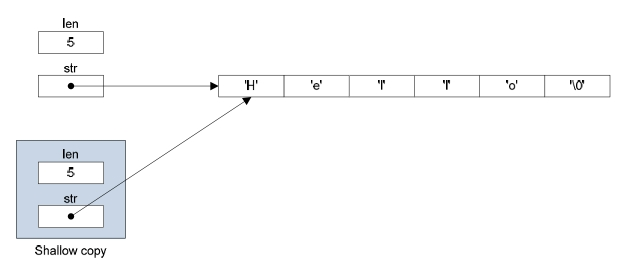
\includegraphics[width=1\textwidth]{pics/shallow_copy.jpg}
			\end{minipage}
			\hspace*{0.5cm}
			\begin{minipage}[t]{9cm}
				\paragraph{Deep-Copy}
					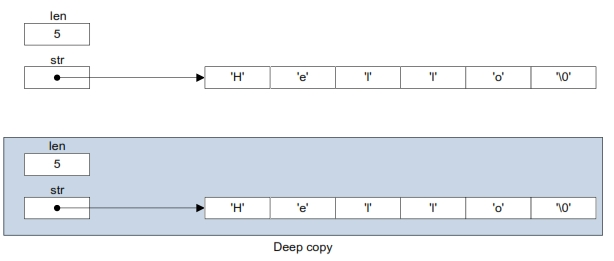
\includegraphics[width=1\textwidth]{pics/deep_copy.jpg}
			\end{minipage}
			
	\subsection{Destruktor \verweiscpp{11.7.2}}
		